\documentclass{exam}
\usepackage{amsmath}
\usepackage{graphicx}
\def\myhrule{\vspace*{0.05in}\lower1ex\null\vadjust{\hrule}}

\pagestyle{head}
\header{\textit{\large Scripps Ranch High Physics Club}}{}{\thepage}
\firstpageheader{\textit{\large Scripps Ranch High Physics Club\myhrule}}{}{\large October 27, 2025 \myhrule}
\begin{document}
    \vspace*{-25px}
    \begin{center}
        \huge \textbf{Newton's Laws}
    \end{center}
    \vspace*{0.05in}
    
    \begin{questions}
        \large
        \question Three blocks $A$, $B$, and $C$ are in contact with each other, 
        and they are at rest on a horizontal surface with negligible 
        friction. The mass of the blocks are given by $m_A$, $m_B$ and 
        $m_C$ respectively. A force pushes block $A$ to the right, and block $A$ exerts a force of magnitude $F$ newtons on $B$. 
        Find the acceleration of each block in terms of $F$ and the three masses\\
        \begin{center}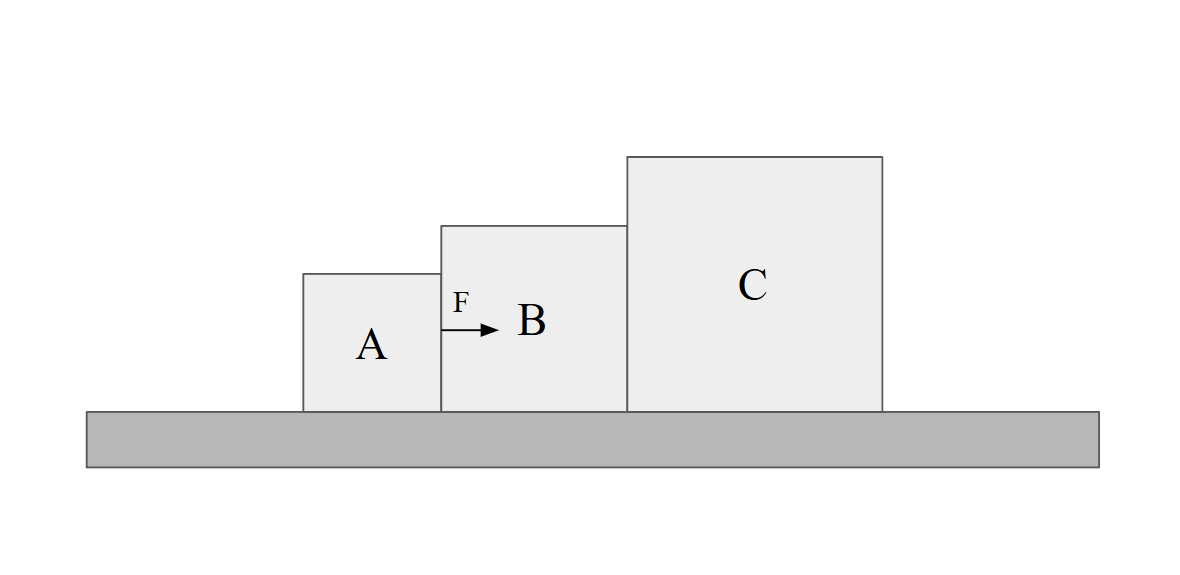
\includegraphics[width=400px]{../assets/blocks.png}\end{center}
        \vspace*{1.4in}
        \question Bob pushes a block of mass $m$ with a constant force of magnitude $F$ newtons. Once the block travels $x$ meters, Bob calculates the velocity at that point to be $v$.
        Suppose Bob were to repeat the experiment, keeping $F$ and $x$ the same, but decreasing $m$ by a factor of $2$. Write what the new final velocity of the block would be in terms of $v$.
        \vspace*{2in}
        \question A block hangs vertically by a rope, with uniform density, attached to a hook as shown. Assuming the weight of the rope is \textbf{not} negligible. Draw free-body diagrams for each of the following points:
        \begin{parts}
            \part The point of the rope attached to the hook
            \part The middle of the rope
            \part The end of the rope attached to the weight
            \part The center of the weight
        \end{parts}
        \begin{center}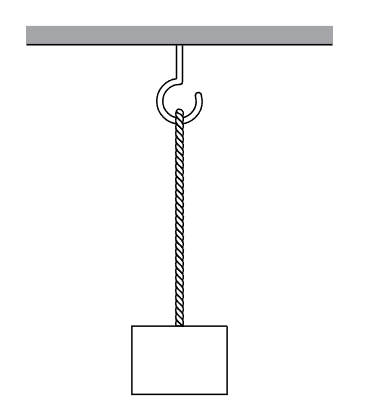
\includegraphics[width=200px]{../assets/hook.png}\end{center}
        \question A passenger in the backseat of a car is thrust to the side of the car when the car takes a sharp turn. Ignoring the friction of the passenger's seat, draw a free-body diagram of the passenger. What newtonian law and physical property is guiding his motion?
        \vspace*{0.5in}
        \question Suppose you were to bring a drone into an elevator and cause it to hover at a constant height from the ground. What would happen if this drone kept hovering as the elevator rose up to a higher level?
    \end{questions}
\end{document}